\chapter{Introduction}
\label{chap:introduction}

Blockchains have enabled a new global market for digital art, allowing artists to publish and sell their work directly to collectors from all over the world, bypassing traditional gatekeepers such as art galleries, auction houses and art dealers. Through chains of cryptographic proofs and consensus protocols which enable public append-only ledgers, blockchains are able to maintain the full history of an artwork's market transactions, from its inception (or \gls{minting}), to its first sale on the \gls{primary market}, and onwards through subsequent transactions on the \gls{secondary market}, and thus natively solve, at least partially, the issue of art provenance, a long-standing problem in the traditional art world. In addition to that, with the use of smart contracts that automatically enforce artist royalties, artists can benefit from a life-long revenue stream, both from \gls{primary sales} and \gls{secondary sales} alike.

As is usual in the art world, when a new technology presents itself, some artists explore its possibilities as an art medium, and blockchain technology was no exception. Artists such as Kevin Abosch, Rhea Myers, Sarah Meyohas, and Sarah Friend, among others, pioneered \gls{conceptual art} using blockchain as a medium, exploring new kinds of interaction between artist, artwork, and collector \cite{rcsBlockchainMedium2022}.

Computational artworks with networking capabilities were made to interact with their environment, and thus evolve over time. However this network capability also brought with it problems. Many code-based artworks become immutable from the moment they are registered on a blockchain, yet the external environment with which they interact keeps changing, and often times those changes are unforgiving for a code-based artefact which cannot mutate to accommodate them, in what can be called a \emph{mutable dependency dilemma}.

This work explores that dilemma, and examines the conservation of networked-based computational art through a technical and cultural lens of \gls{web3}, which is native to the blockchain and crypto community.

This thesis contains many terms which were born out of the crypto community and may be unfamiliar to the reader. Even the term \emph{crypto} itself, with its Greek origins, has been adopted by the cryptocurrency community, thus appropriating a term which until recently had been used mostly by the cryptography community. For this reason this document contains an extensive glossary, starting from page \pageref{sec:glossary}, where many of the terms are defined.

\section{Motivation}

To better understand my motivation for this work, as well as contextualise some of the research and development decisions made during the study, it is helpful for the reader to review a brief timeline of my personal experience in the crypto space and how it led to this research topic. Due to its personal nature, I took the liberty of using a more informal tone in this section.

\subsection*{Bitcoin}

I first came across Bitcoin in 2011, and experienced the basic use case of installing the Bitcoin-QT software on my laptop and receiving a small transaction (0.02 BTC) from a public faucet ran by early bitcoin developer Gavin Andersen \cite{lucasHowGavinAndresen2022}. As many people at that time, I failed to understand the significance of such a transaction. From a user experience (\indexacronym{ux}) perspective it was underwhelming.  The interface was rudimentary, and the transaction took a while to appear as confirmed. Paypal was miles ahead, or so I thought. This mis-judgement of the merits of the technology due to a very limited understanding, or even complete ignorance, of such a technology is unfortunately very common in the crytocurrency space.

It wasn't until 2013 that I looked into Bitcoin again. This time I read the Bitcoin whitepaper \cite{nakamotoBitcoinPeertopeerElectronic2008} and my world view changed. Technologically the proposition was simple: here is a piece of software which, if enough people run it on their own devices, and adopt it as a legitimate way to communicate value with others, has the potential to redefine the relationship between money, the state, and the people.

As an anarchist sympathetic with the anti-capitalist movement, I brushed aside the fact that Bitcoin was firmly rooted in a capitalist culture, because it also represented a very tangible step away from a financial system which I saw as irreparably corrupt. I became an advocate, organising Bitcoin meetups in Macau \cite{BitcoinMacau2024}, delivering public courses \cite{mouraUSJHoldCourse2021}, appearing in interviews to the media \cite{tdmportuguesenewsprogramsReportagemJornalistaLina2015} \cite{reisBitcoinDuasFaces2017} and generally being very active in the Bitcoin community.

\subsection*{Ethereum}

In January 2014, when Ethereum was announced as a concept by Buterin \citeyear{buterinEthereumNextGenerationCryptocurrency2014}, I was instantly impressed. Bitcoin always had basic scripting capabilities baked into its transaction processing logic \cite{ScriptBitcoinWiki2024}, but to take what was mostly a transactional ledger technology and enhance it with a Turing-complete runtime was going to open a world of possibilities. But perhaps even more importantly, Ethereum was also marketed as a decentralised platform where \emph{\gls{code is law}}, a concept which deeply resonated with me. The idea of encoding governance into public, immutable, and self-enforceable rules seemed like a silver-bullet against corruption.

In 2016, a bug was exploited in a smart contract of a DAO which held around 14\% of all ETH in circulation \cite{morrisCoinDeskTurns102023}. Under the \emph{code is law} philosophy, the exploiter only followed the rules of the code, and was therefore the rightful owner of the drained funds. However the Ethereum core developers dismissed the \emph{code is law} mantra and proposed a hard-fork of the blockchain \cite{buterinCRITICALUPDATERe2016} to effectively reverse the attack, salvaging the funds from the hands of the hacker and returning it to their original owners. This was an extremely controversial decision, especially for a space where trustlessness, censorship-resistance, and immutability of transactions are core elements. To make matters worse, in addition to such a significant u-turn in philosophy, the way in which matters were dealt with, much of which documented by an anonymous member of the community \cite{yourstruly1DAOHistoryIt2018}, was very disappointing. Even if Ethereum Classic carried on with the original chain and philosophy \cite{CodeLaw2022}, I was too disillusioned with the crypto space and took a step back.

I should note that more recently I changed my stance regarding \emph{code is law}, as will be explained later.


\subsection*{Tezos}

In the summer of 2017 I came across Tezos, a project still in its inception stage, but which was planning to build a self-amending blockchain with a well designed governance system built into protocol, giving its token holders voting power on updates to the protocol itself \cite{goodmanTezosSelfamendingCryptoledger2014a} . 


This was exciting to me because it promised to address the main problem that had led me to exit the Ethereum ecosystem. In addition to that, it would also use a proof-of-stake consensus algorithm from day one, resulting in a much more energy efficient and ecologically friendly blockchain.


Ironically, after delays due to extensive governance issues and disputes between the project co-founders and the president of the Tezos Foundation, who eventually stepped down \cite{irreraExclusiveTezosFounders2017}, Tezos finally launched in September 2018 \cite{daleBillionTezosBlockchain2018}. The delay in the launch is sometimes referred to as a reason why Tezos fell behind other projects in the crypto space, both in terms of developer mindshare as well as overall relevance, in what is a very competitive market.

The following three years saw a modest amount of development around Tezos especially in the areas of \gls{decentralisedfinance} and gaming, however adoption of the chain remained relatively low, as measured by the low transaction volume recorded on the chain, encouraging detractors to classify it as a \emph{\gls{ghost-chain}}, as an analogy to a ghost town. In March 2021 all that was about to change.


\subsection*{Hic Et Nunc (HEN)}


Hic et Nunc (\indexacronym{hen}) was an NFT marketplace developed by Brazilian developer Rafael Silva, a former social scientist from Brasília. Lima launched HEN on the Tezos blockchain in March 2021, becoming the first to do so on that chain, and in the process beating rival marketplace Kalamint, who was still in closed beta.

At a time when the NFT market was experiencing a boom cycle \cite{haywardBiggestCryptoStory2021} , many artists, especially those from the Global South, were priced out of the fast increasing gas prices on Ethereum, on account of the high demand for block space. At the same time environmentally conscious artists raised concerns about Ethereum's high carbon footprint, since at that time it still operated on a \gls{proofofwork} consensus algorithm \cite{lemercierProblemEthereumCryptoArt2021}. With Tezos offering very low transactions costs, and also being environmentally friendly due to its \gls{proofofstake} consensus algorithm, HEN's launch on Tezos provided a solution for these two groups of artists. Prominent artists like Joanie Lemercier and Mario Klingemann quickly saw the potential of the platform and started promoting it amongst their peers. With an iconic minimalistic and raw interface, the platform invoked an underground culture of experimental and avant-garde digital art. It also intentionally lacked any kind of artist signup process or similar kinds of gatekeeping. Anyone with as little as 0.5 XTZ (approximately \$2.5 USD at the time) in a Tezos wallet could mint an artwork on HEN. After only a few weeks, HEN rose in popularity and became a boiling pot of creativity and experimentation \cite{evansBrazilDIYEcofriendly2021}.

Pioneering museum strategist, and curator Diane Drubay, reflecting on the HEN experiment, stated:

\begin{quotation}
``In March 2021, if you were minting on hic et nunc, you had no choice but not to sleep anymore. It was hectic and so beautiful! The energy was thrilling and every day was a new adventure.'' \cite{drubayHowHicNunc2021}
\end{quotation}


By May 2021 HEN overtook OpenSea, the largest NFT marketplace in Ethereum, in number of active users \cite{nelsonWhereAreYour2022} \cite{evansBrazilDIYEcofriendly2021}. This sudden rise in usage can be clearly observed on the number of transactions and smart contract calls on the Tezos blockchain which started climbing just after March 2021, see \autoref{fig:tezos-tx-vol}.

Each NFT platform on Tezos adopts a token name for its NFTs, and Rafael Lima named the HEN tokens: \gls{OBJKT}, which is not an acronym.
The term OBJKT was later \emph{adopted} by a rival marketplace, objkt.bid, which then became objkt.com, and which is today the largest NFT marketplace in the Tezos ecosystem.

\begin{figure}[h]
    \centering
    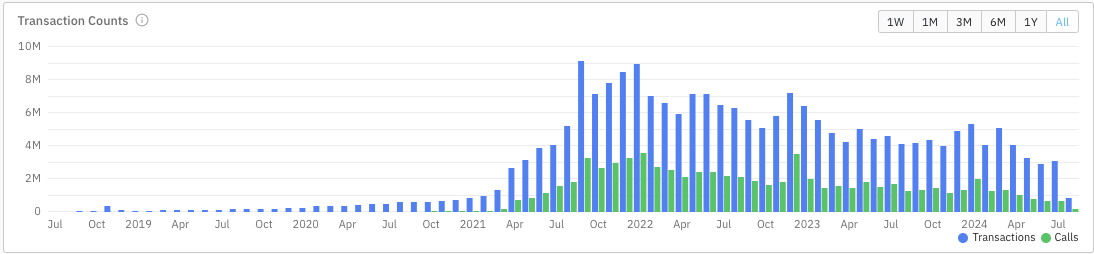
\includegraphics[width=\linewidth]{chart-tezos-tx-volume.png}
    \caption[Transactions per month on Tezos blockchain]{Transactions per month on Tezos blockchain (Jul 2018 - Jul 2024). Source: https://tzstats.com/}
    \label{fig:tezos-tx-vol}
\end{figure}

\subsection*{Networked OBJKTs and ``Self-Aware'' Artworks}

HEN supported the minting of OBJKTs using a variety of file formats, and one of those format was SVG (mimetype \texttt{image/svg+xml}). The SVG file standard allows for the embedding of JavaScript code, which is executed when rendering the file on a web browser.  On 14 Mar 2021 French artist Lionel Radisson minted the first OBJKT with embedded JavaScript, ``The Magician''  \cite{makio135Magician2021}, and other artists quickly followed and started minting dynamic code-based artworks. Ricardo Cabello (a.k.a mrdoob), creator Three.js, minted the interactive game ``Jumpy Dot'' \cite{mrdoobJumpyDot2021} which became the first in-browser interactive game minted as an NFT \cite{rusherWhatDoesIt2021}.

\begin{figure}[H]
    \centering
    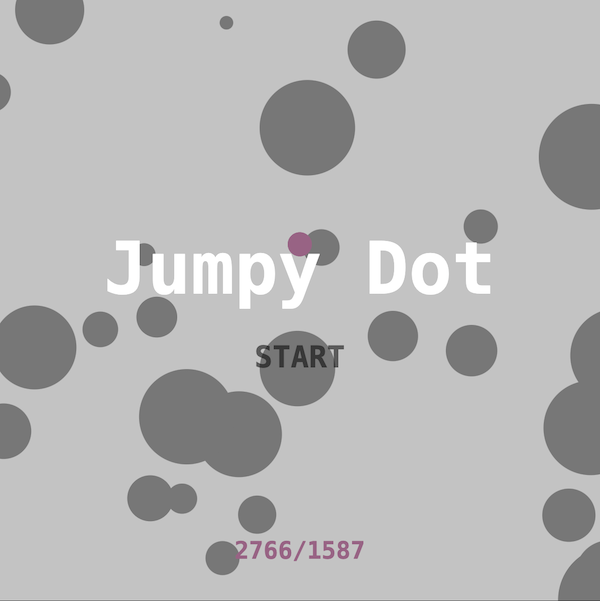
\includegraphics[width=0.5\textwidth]{jumpydot-play.png}
    \caption[``Jumpy Dot'' by mrdoob]{``Jumpy Dot'' by mrdoob}
    \label{fig:jumpydot}
\end{figure}


Soon afterwards, the first few OBJKTs that made network (\indexacronym{http}) requests appeared. The first ones only loaded external webpages, or even played with recursion by loading the HEN website itself, but then these were quickly followed by OBJKTs that made calls to public \indexacronym{api}s.

It was at this stage that Mario Klingemann (a.k.a. quasimondo) minted a conceptual OBJKT, ``Planned Obsolescence'', which makes an HTTP request to a blockchain indexer API, giving it access to a real-time list of collectors of that OBJKT. The piece started with a misty, dreamlike landscape painting as a background, but each time a new collector bought the OBJKT, the artwork's JavaScript code would retrieve the collector's Tezos wallet address from the API, and displayed it on top of the landscape, increasingly obscuring it, see \autoref{fig:plannedobsolescence}.

\begin{figure}[H]
    \centering
    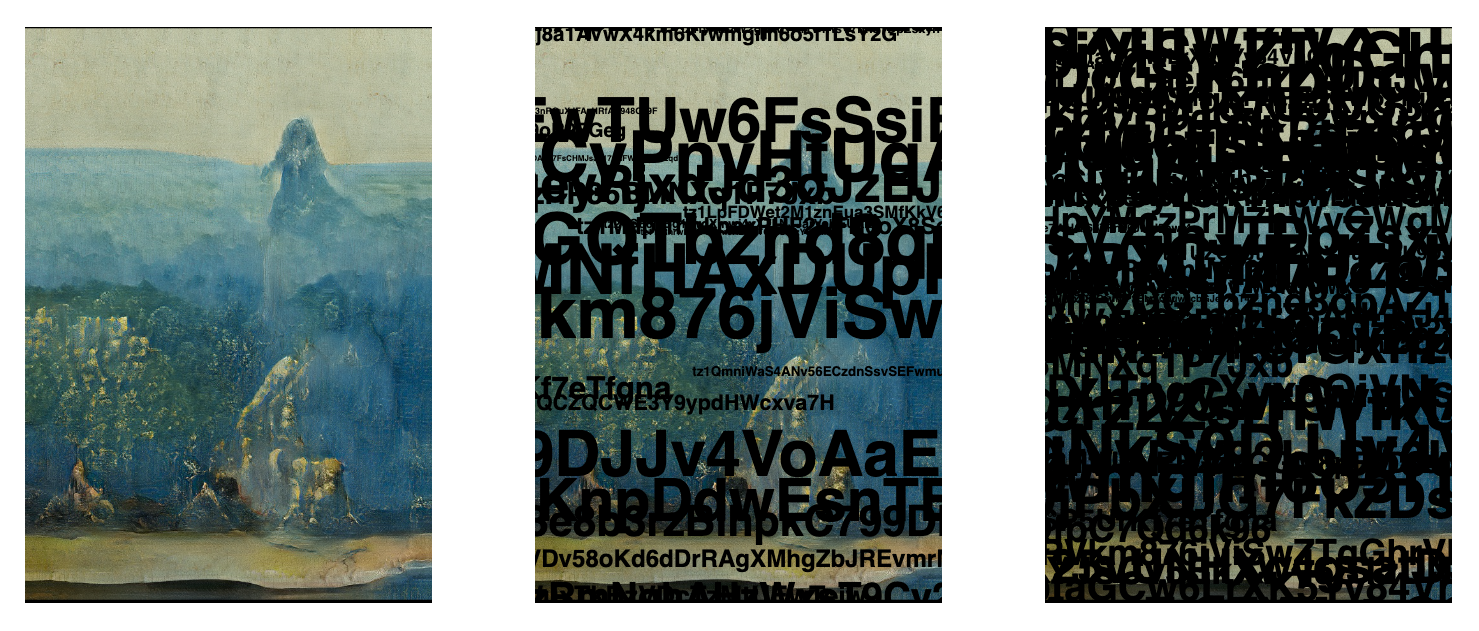
\includegraphics[width=\textwidth]{planned-obsolescence.png}
    \caption[``Planned Obsolescence'' by quasimondo]{Three renderings of ``Planned Obsolescence'' by Mario Klingemann (quasimondo)}
    \label{fig:plannedobsolescence}
\end{figure}


This kickstarted a wave of self-referential, some would even call it ``self-aware'' artworks, which also have the property of evolving over time. Many of which will be reviewed later in this manuscript.

This concept of ``self-awareness'' of an artwork struck a chord in me, and I decided to study it in detail. It soon became clear that this kind of artwork faces a number of challenges, which are discussed in \autoref{sec:challenges}.


\subsection*{HEN Discontinuation}
\label{sub:teia}

For reasons which are outside of the scope of this thesis, but which are reported at length in online articles \cite{straeubigHENTimelineHentimeline2024} \cite{siqueiraHicNuncStory2021a} \cite{tezosHistoryTeiaArt2022} \cite{smithHicNuncPart2022}, on November 11 2021, only 9 months since its launch, Rafael Lima decided to discontinue HEN. Without warning, the webserver which served the website's \indexacronym{ui} was taken down (\texttt{hicetnunc.xyz}), and the official twitter account was changed to show the message "discontinued".

\begin{figure}[h]
    \centering
    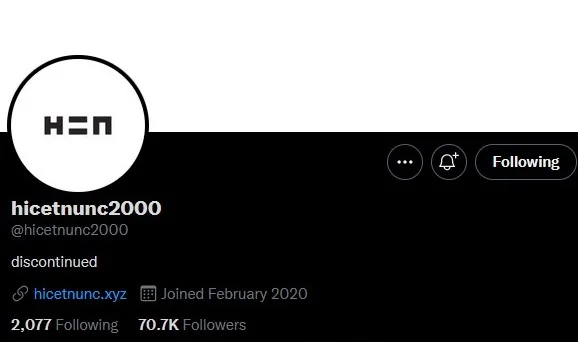
\includegraphics[width=0.75\textwidth]{discontinued.png}
    \caption[``discontinued'' by Rafael Lima]{`discontinued'' by Rafael Lima. Source: https://t.ly/PtiOd}
    \label{fig:discontinued}
\end{figure}

Fortunately, Lima had followed the Web3 ideals of decentralisation and trustlessness when he designed and built HEN. The source code of the website's UI was open source and hosted on GitHub, and the smart contracts that the platform relied on were still operational on the Tezos blockchain, and did not contain any \emph{kill switch}, therefore they formed a sort of public utility infrastructure beyond the reach of their own creator. The artwork media assets were available on a public storage network (IPFS) and therefore were publicly accessible as well.

The community that had formed around HEN quickly entered into action and in only a few hours several clones of the UI were setup online, in what the community calls ``mirrors'', allowing users to continue minting, and collecting OBJKTs just as they did before. Efforts were made to ensure the continuity of the media assets on IPFS, and this was also achieved successfully.

After some time, the community converged on a particular HEN mirror, and after requests from Lima to not use the name HEN, the community renamed it Teia ("web" in Portuguese, in a gesture of respect to the Brazilian roots of the original project). And thus the Teia community was formed and the new website domain adopted: \texttt{teia.art}.

Today, Teia operates as a Decentralised Autonomous Organisation \gls{dao}, is legally established as non-profit organisation, and continues to operate thanks to a team of volunteers.

For disclosure, I am a member of the Teia core team, which consists of 19 community members who currently operate the platform and oversee the treasury my means of voting on a multisig smart contract on Tezos. The roadmap is to migrate the governance to a much larger DAO structure, where thousands of users who currently hold TEIA governance tokes, which were distributed based on their usage of the platform and contributions to project, can vote on proposals related to the project.

As a Teia team member, my focus is the preservation of code-base OBJKTs, which are called Interactive OBJKTs in the platform's terminology.



\section{Challenges}
\label{sec:challenges}

The biggest challenge facing a networked artwork is a mismatch between the immutability of the NFT and the fast changing nature of the environment in which it operates. This is not a problem for the vast majority of artworks, because they represent static assets, such as image, video, or sound files. As long as their file formats are supported by modern web browsers then they should continue to work for a reasonable amount of time.

Code-based artworks, if they contain all the required software dependencies and assets, such that you can successfully render them on an off-line device, should in theory also last a reasonable amount of time, notwithstanding the need for emulation at a later stage.

However an artwork that requires data from external sources runs a number of risks, because the data source can:

\begin{itemize}
    \item make changes to the data structure that it returns (for example, API version upgrades)
    \item phase out a particular set of resources
    \item change the URI path of its resources
    \item limit access to its resources
    \item simply stop functioning (for example, organisation out of business, or project abandoned)
\end{itemize}

Any of these events would pose a problem to a piece of software which cannot be modified to accommodate those changes. This mismatch between an immutable software artifact and an evolving environment in which it depends will be called the \emph{mutable dependency dilemma}.

The long-term preservation of the digital assets required by the artworks is also problematic. As will be discussed in the following chapter, there are several approaches, each with pros and cons, however this is area of heated debate in crypto art.

An additional challenge is that these artworks often lack the required metadata to differentiate networked, from non-worked code-based artworks. This makes it difficult for a conservator to identify which artworks may need attention.

Finally, although not directly related to conservation, any code-base artwork carries a security risk to those who access it, due to software vulnerabilities as well as potentially malicious code.

\section{Goals}

In order to address the challenges outlined above, and from an information systems (\indexacronym{is}) perspective, two main goals arise for this work:

\begin{itemize}
	\item To design and implement a sustainable IS that can support the long-term preservation of networked crypto art
	\item To contribute to the body of knowledge in the area of networked crypto art conservation
\end{itemize}

The reason why sustainability is explicitly included as an objective is because it is a requirement to support \emph{long-term} preservation, and even though there are many types of sustainability which should be considered, in this context the key factor is economic sustainability.

\section{Contributions}

The principal contribution of this work is an open-source web-based software artifact, \texttt{ARKIVO}, which:

\begin{enumerate}
	\item indexes all code-based OBJKTs minted on the HEN smart contract
	\item classifies the artworks according to their properties
	\item executes and snapshots network calls initiated by the artworks during their execution
	\item takes screenshots of the artwork during execution
	\item stores a copy of all artwork assets
\end{enumerate}

\vspace{0.5cm}

The system is live, accessible at \texttt{https://arkivo.art} and its source code can be accessed from:

\texttt{https://github.com/seda-studio/arkivo}

\vspace{0.5cm}

A secondary contribution is the proposal and implementation of a new method for the creation of mutable crypto art based on blockchain version control, which can be considered a kind of preventive conservation technique.

Thirdly, a physical device is proposed, intended to be run from home, that contributes to the storing of the artwork digital assets. This component is key for the decentralisation, and long term economic sustainability of the project. 

\vspace{0.5cm}

In addition to these artifacts, this work makes the following contributions to the body of knowledge:

\begin{enumerate}
    \item Taxonomy and classification of code-based crypto art
    \item Identification of networked OBJKTs minted on the HEN smart-contract
    \item Analysis of the total asset size, and rate of growth of all code-based OBJKTs minted on the HEN smart-contract
    \item Case studies of restoration attempts of a sample of networked OBJKTs
    \item A set of best practices for artists who plan to create networked artworks
\end{enumerate}


\section{Definitions}
\label{sec:definitions}

Although a comprehensive glossary is included at the end of this thesis, see page \pageref{sec:glossary}, this section outlines the precise definitions and scope of some of the key terms used in this thesis.

\vspace{0.5cm}

\textbf{crypto art} - this refers to any artwork which is registered on a blockchain as an NFT, and which exists purely in digital format, without any physical components.

\vspace{0.5cm}

It should be noted that this last assumption is really more a delimitation of scope for this work rather than a universal definition of crypto art, some of which can indeed have physical components. It is important to clearly define this aspect of the work at the outset, as the conservation of physical artifacts requires a very different approach to digital-only artifacts.

\vspace{0.5cm}

\textbf{code-based art} - this refers to any artwork which is created with computer code and which requires a computer to execute it in real time in order to render the artwork. The term \emph{encoded} is also used in some of the literature. In the case of this study, it specifically refers to artworks that use web technologies (HTML, CSS, JavaScript, SVG, and others) which are rendered in real time by the viewer's web browser.

\vspace{0.5cm}

It follows then that \emph{code-based crypto art} refers to artworks based on computer code which are registered as NFTs on a blockchain.

\vspace{0.5cm}

\textbf{networked art} - a specific kind of code-based art which initiates network requests, normally via HTTP or HTTPS, to an external URL which is outside of its own artifact directory (identified by a specific directory URL). Any network requests made for internal assets (which are relative and internal to the artifact's directory) are excluded from this definition.

\vspace{0.5cm}

This is an important distinction, because any code-based artifact will normally make several HTTP requests to load local assets (fonts, css files, media files) but as long as these are stored within the artifact's own directory they should always be available to the artifact, therefore not posing a \emph{mutable dependency dilemma}.

\vspace{0.5cm}

\textbf{conservation} - ``Conservation encompasses all those actions taken toward the long-term preservation of cultural heritage. Activities include examination, documentation, treatment, and preventive care, supported by research and education.''  \cite{WhatConservation}

\vspace{0.5cm}

Regina Harsanyi, a preventive conservator of time-based media who works extensively with blockchain related artworks, during an interview for this study highlighted that the code of ethics followed by conservation professionals is also key to the definition of the term \cite{americaninstitutefrorconservationCodeEthicsGuidelines}.

\vspace{0.5cm}

The terms conservation and preservation are often used interchangeably in the digital art literature, and definitions are often contradictory. For the purpose of this study, the following definition is proposed:

\vspace{0.5cm}
\textbf{preservation} - the goal of ensuring that cultural heritage remains accessible to future generations.

\vspace{0.5cm}

In summary, whereas preservation is the goal, conservation deals with the methods and techniques to achieve it.

\vspace{0.5cm}

\textbf{artifact} - ``an object made by a human being, typically an item of cultural or historical interest'' \cite{OxfordAdvancedLearner}. However it should be noted that this term is used extensively in this thesis in two distinct contexts:

\begin{enumerate}
    \item the software system, \texttt{ARKIVO}, which was developed as part of this research and constitutes its main contribution;
    \item the crypto artworks which are the subject of the conservation techniques which this research explored.
\end{enumerate}

\vspace{0.5cm}

It is somewhat unfortunate that this name collision occurred for these two types of artifacts, however both are used extensively in the Design Science Research literature, which was the methodology adopted for this study, as well as in the existing software systems that already deal with crypto artworks. It is hoped that, when reading the text, the reader will be able derive which type it is based on its immediate context. It is also for this reason that the other common use of this term, as a kind of error or anomaly, was avoided. 

\section{Delimitation of Scope}

The focus of this research is on the conservation of networked crypto art, however the scope of the artifact created for the study is delimited to OBJKTs minted on the HEN smart contract on the Tezos blockchain, and thus the analysis, discussion and conclusion sections of the work will also be delimited to that scope.

Having said that, \autoref{sec:survey-crypto-art} (\nameref{sec:survey-crypto-art}, page \pageref{sec:survey-crypto-art})  will provide a broader view and review artworks that may fall outside this scope, in order to provide additional context to the area of crypto art. Namely it will review artworks minted in other platforms and blockchains.

\section{Relevance of Research}

Although the scope of the research may seem narrow, the subject on which it focuses is of significant relevance to the cultural heritage of crypto art.
HEN, even if short-lived, is widely acknowledged to represent one of the most important cultural events and social experiments that happened in the world of crypto art, not only because of the art, but also for demonstrating the importance of web3 principles \cite{rcsEarlyDaysHic2023} \cite{baileyHicNuncBrings2021} \cite{drubayHowHicNunc2021}.
In addition to this, networked crypto art is a type of art that artists pioneered on HEN and hence of the utmost importance to be preserved.

\section{Structure of the Thesis}

This chapter introduced the motivation for this study, identified the main challenges of networked crypto art and outlined the goals and contributions of the study, followed by definitions of key terms, as well as determining the scope of the study. The remainder of the thesis is structured as follows:

Chapter 2 reviews related work, including digital art conservation theory, existing archival standards and tools, the technical architecture of existing HEN OBJKTs, provides a survey of representative artworks and proposes a tentative taxonomy of code-based crypto art.

Chapter 3 introduces the research questions and describes the methodology used in this study, namely Design Science Research, as well as the methods and tools used as part of the research and development.

Chapter 4 provides a detailed account of the prototyping phases when developing the artifact.

Chapter 5 describes the systematic analysis and evaluation of the artifact. It also provides a discussion on the lessons learned during its development.

Chapter 6 introduces a new paradigm for the creation of mutable and evolving crypto art, and discusses other techniques for the conservation of this kind of art.

Chapter 7 summarises the main points of the thesis, provides a set of recommended best practices for creating code-based crypto art, and outlines ideas for future work.
